\documentclass[a4paper, UTF8, twocolumn ]{ctexart}
% \documentclass[a4paper, UTF8]{ctexart}
\usepackage{graphicx}
\usepackage{amsmath}
\usepackage{amssymb}
\usepackage{paralist}
\usepackage[
colorlinks,
linkcolor = black
]{hyperref}

\usepackage{fancyhdr}                                
\usepackage{lastpage}                                           
\usepackage{layout}                                                                          

\linespread{1.56}
\columnsep = 15pt
\columnseprule=1pt
\begin{document}

\title{\huge{基于正态分布概率计算和支持向量机计算的WiFi定位技术}}
\author{北京优锐科技有限公司\ 丁贵金\ 朱韬\ 袁万尚}
% \author{北京优锐科技有限公司\ 朱韬}
\date{\today\\*\ \hrule}
\maketitle

%%%%%%%%%%%%%%%%%%%%%%%%%%%%%%%%%%%%%%%%%%%%%%% 

\begin{abstract}
  基于概率和支持向量机原理的 WiFi定位技术,不需要依赖专用设备,部署简单使用便捷,对环境无强制依赖,可以在复杂 WiFi 环境下实现移动设备精确定位。该 WiFi 定位技术的核心原理是支持向量机,辅助正态分布的概率计算来优化支持向量机计算过程。
  \par
  本文针对的设备:是带有WiFi功能的移动设备。针对的环境:是分布着大量WiFi接入设备的室内环境。实现的主要目标:是通过WiFi移动设备,在分布着大量WiFi接入设备的室内环境中,实现精确定位。
  \par
  \noindent{\textbf{关键词}:}WiFi定位,室内定位,支持向量机。
\end{abstract}

%%%%%%%%%%%%%%%%%%%%%%%%%%%%%%%%%%%%%%%%%%%%%%% 

\section{引言}
本文的“名词、概念和常识说明”部分,主要解释全文中出现的各种专用名词,涉及到的所有概念,以及阅读本文所需的技术常识。“实现方法”部分则具体阐述技术实现过程,“讨论”部分主要分析了实现过程中可能出现的各种问题,以及处理问题的方法。“技术创新”部分具体说明该技术的先进性,与同类技术相比下的优势,“应用前景”部分介绍了该技术实际应用的具体形式,以及对采用该技术的行业所产生的积极作用。

%%%%%%%%%%%%%%%%%%%%%%%%%%%%%%%%%%%%%%%%%%%%%%% 

\section{名词、概念和常识说明}
\subsection{定位空间(CR)}
定位空间(calibration room),指的是提供定位功能的空间。例如采用WiFi定位的公司内部空间,公司外部无限大的空间就是不可定位空间。如图\ref{fig:CR}:
\begin{figure}[!ht]\centering
  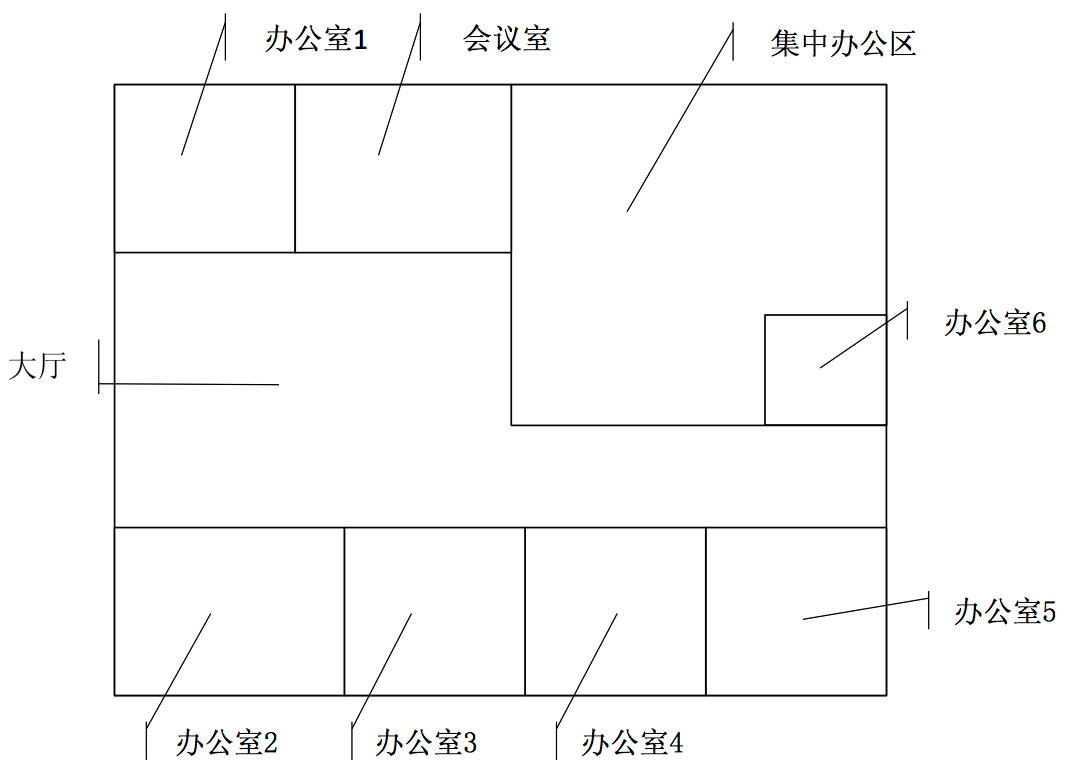
\includegraphics[keepaspectratio, scale=0.2]{no2.png}
  \caption{定位空间示例图\label{fig:CR}} 
\end{figure}
\subsection{移动终端设备}
本文中的“移动终端设备”,是指拥有WiFi连接能力的移动设备,如有WiFi功能的智能手机、平板电脑和其他便携的移动终端设备。
\subsection{WiFi接入设备(AP)}
提供WiFi接入服务的硬件设备,如无线路由器。本文中对WiFi接入设备的要求,是必须能够被移动终端设备识别到的WiFi接入设备。
\subsection{AP名(MAC)}
本文中所用AP名就是AP的MAC地址,是WiFi接入设备的唯一标示。
\subsection{AP信号强度(RSS)}
AP信号强度,是移动终端设备对WiFi接入设备信号强度的识别结果。该结果是一个从0到-100的值,该值是一个指数值,代表信号的强度指数,并不是真正的物理信号量。不同的移动终端设备,对同一个WiFi接入设备,信号强度值的识别结果是不同的。
\subsection{AP信号强度平均值(mRSS)}
同一个移动终端设备,对同一个WiFi接入设备,每次信号强度的识别结果也是不同的。一个移动终端设备,对同一个WiFi接入设备,进行多次采集,识别到一组信号强度,对该组信号强度的求平均值,就得到了信号强度平均值,计算公式如下:
\begin{equation}\centering
  mRSS=10\lg\left(\frac{1}{N}\sum^{N}_{i=1}10^{\frac{RSS_{i}}{10}}\right)
\end{equation}
N为该组信号强度的个数。
\subsection{WiFi接入设备数据}
WiFi接入设备数据包括,WiFi接入设备名MAC地址,和WiFi接入设备识别到AP的信号强度。
\subsection{待定位点(LP)}
带定位点,是指一个移动终端设备,出现在定位空间内,该移动终端设备自身的位置。
\subsection{定位区域(value)}
定位空间是一个完整的封闭空间,要在这个空间内实现WiFi定位,就必须将这个完整的空间划分为多个小区域,每个区域都有一个ID。如图\ref{fig:value}:
\begin{figure}[!ht]\centering
  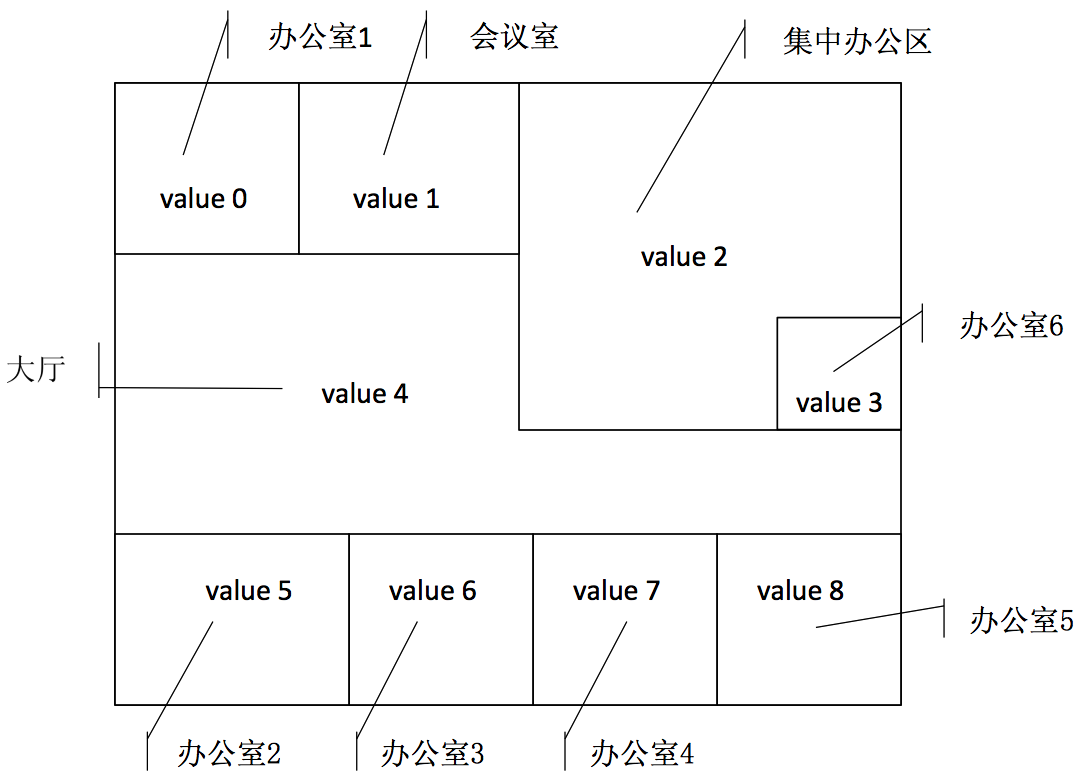
\includegraphics[keepaspectratio, scale=0.2]{no3.png}
  \caption{定位区域示意图\label{fig:value}} 
  其中value 0中0就是该定位区域的ID。
\end{figure}
\subsection{定位校准点(CP)}
在定位区域中,指定一个位置点,这个点就是定位校准点。一个定位区域内可能会有多个定位校准点,在这些点上所识别到的WiFi接入设备数据,都输入这个定位区域的定位区域数据。如图\ref{fig:CP}:
\begin{figure}[!ht]\centering
  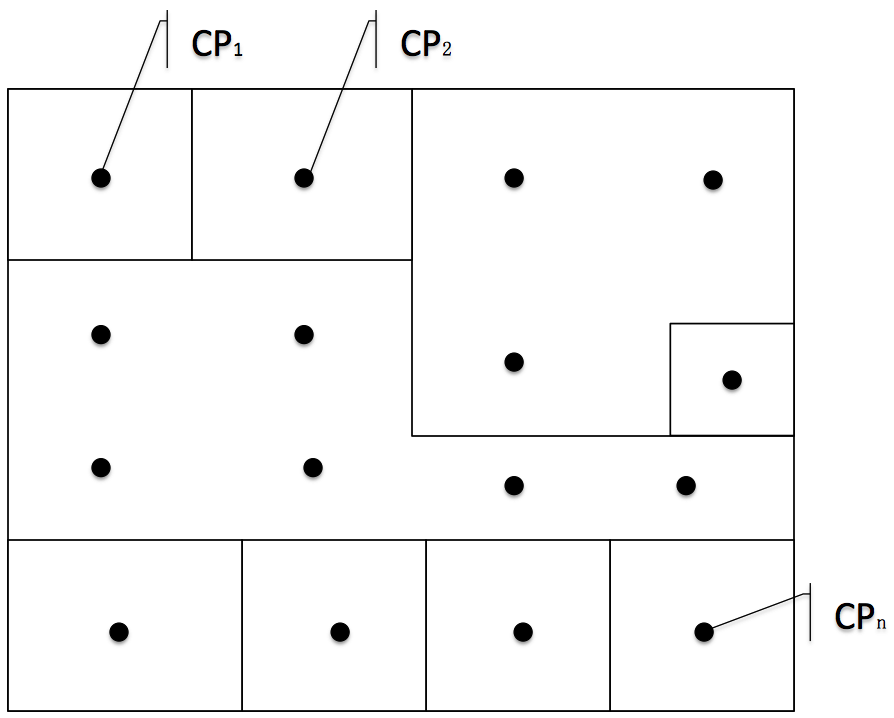
\includegraphics[keepaspectratio, scale=0.2]{no4.png}
  \caption{定位校准点示意图\label{fig:CP}} 
\end{figure}
\subsection{定位区域数据}
在定位区域内的定位校准点上,一次采集到的WiFi接入设备数据,就是定位区域采集数据。该数据的标示是区域ID,内容是WiFi接入设备数据。如下表所示:
\begin{equation}
  \begin{array}{c|c|c}
    Value & AP_{i} & RSS_{i}\\
    \hline
    0 & MAC_{1} & RSS_{1}\\
    0 & MAC_{2} & RSS_{2}\\
    0 & MAC_{3} & RSS_{3}\\
    0 & MAC_{4} & RSS_{4}\\
    0 & MAC_{5} & RSS_{5}\\
    ... & ... & ...
  \end{array}
\end{equation}
多次采集定位区域数据后,一个AP会对应多个RSS值。如下表所示:
\begin{equation}
  \begin{array}{c|c|c}
    Value & AP_{i} & RSS_{i,n}\\
    \hline
    0 & MAC_{1} & RSS_{1,1} ... RSS_{1,2} ... RSS_{1,n}\\
    0 & MAC_{2} & RSS_{2,1} ... RSS_{2,2} ... RSS_{2,n}\\
    0 & MAC_{3} & RSS_{3,1} ... RSS_{3,2} ... RSS_{3,n}\\
    0 & MAC_{4} & RSS_{4,1} ... RSS_{4,2} ... RSS_{4,n}\\
    0 & MAC_{5} & RSS_{5,1} ... RSS_{5,2} ... RSS_{5,n}\\
    ... & ... & ...
  \end{array}
\end{equation}
\subsection{校准数据}
校准数据,是对所有定位区域多次采集到的数据,整理计算后的结果。如下表所示:
\begin{equation}
  \begin{array}{c|c|c|c}
    Value(n) & AP_{i} & mRSS_{n} & \sigma_{n,i} \\
    \hline
    0 & MAC_{1} & mRSS_{1} & \sigma_{0,1} \\
    0 & MAC_{2} & mRSS_{2} & \sigma_{0,2} \\
    0 & MAC_{3} & mRSS_{3} & \sigma_{0,3} \\
    0 & MAC_{4} & mRSS_{4} & \sigma_{0,4} \\
    0 & MAC_{5} & mRSS_{5} & \sigma_{0,5} \\
    ... & ... & ... & ...\\
    1 & MAC_{1} & mRSS_{1} & \sigma_{1,1} \\
    1 & MAC_{2} & mRSS_{2} & \sigma_{1,2} \\
    1 & MAC_{3} & mRSS_{3} & \sigma_{1,3} \\
    1 & MAC_{4} & mRSS_{4} & \sigma_{1,4} \\
    1 & MAC_{5} & mRSS_{5} & \sigma_{1,5} \\
    ... & ... & ... & ...
  \end{array}
\end{equation}
Value是定位区域,n代表不同定位区域的ID号。AP是收集到的所有WiFi接入设备名,mRSS是该WiFi接入设备被识别到的信号强度平均值,i代表不同AP的序号,$\sigma_{n,i}$代表对应一个定位区域中一个AP的信号强度标准差。
\subsection{待定位数据}
移动设备在待定位点,某一时刻采集到的WiFi接入设备数据。如下表:
\begin{equation}
  \begin{array}{c|c}
    AP_{i} & RSS_{i}\\
    \hline
    MAC_{1} & RSS_{1}\\
    MAC_{2} & RSS_{2}\\
    MAC_{3} & RSS_{3}\\
    MAC_{4} & RSS_{4}\\
    MAC_{5} & RSS_{5}\\
    ... & ...
  \end{array}
\end{equation}
AP是识别到的所有WiFi接入设备名,RSS是识别到的所有WiFi设备的信号强度。
\subsection{概率}
\subsubsection{正态分布}
正态分布是一种常用的概率分布函数,本文阐述的WiFi定位技术,在实现过程中采用了这种数学方法。公式如下:
\begin{equation}
  Pr_{i}=\frac{1}{\sqrt{2\pi}\sigma_{i}}e^{\frac{-(RSS_{i}-mRSS_{i})^{2}}{2\sigma_{i}^{2}}}
\end{equation}
\subsubsection{概率值(Pr)}
本文中所讲的概率值,是指一个待定位点,出现在某一定位区域中的概率。
\subsection{支持向量机(SVM)}
支持向量机,是一种机器学习原理,是采用数学方法,实现对某种向量值进行特定分类的工具。
\subsubsection{样本}
本文所说的样本,是指WiFi接入设备的数据。
\subsubsection{样本空间}
多个样本生成的集合,叫做样本空间。
特征向量
本文所说的特征向量,是指可以代表一个定位区域的样本。是校准数据中,一个定位区域中所有样本的子集。
\subsubsection{核函数}
核函数,是指支持向量机所采用的某种特征向量训练模式。本文中的核函数采用RBF核函数,采用该核函数时,需要提供一个高斯参数$\sigma$作为训练调优参数,默认值使用0.75。
\subsubsection{惩罚因子C}
惩罚因子,是指在支持向量机计算中,分割两个样本空间时,对不可分样本的包容程度。默认值1.0。


%%%%%%%%%%%%%%%%%%%%%%%%%%%%%%%%%%%%%%%%%%%%%%% 

\section{实现方法}
\subsection{总体流程}
如图\ref{fig:no11}
\begin{figure}[!ht]\centering
  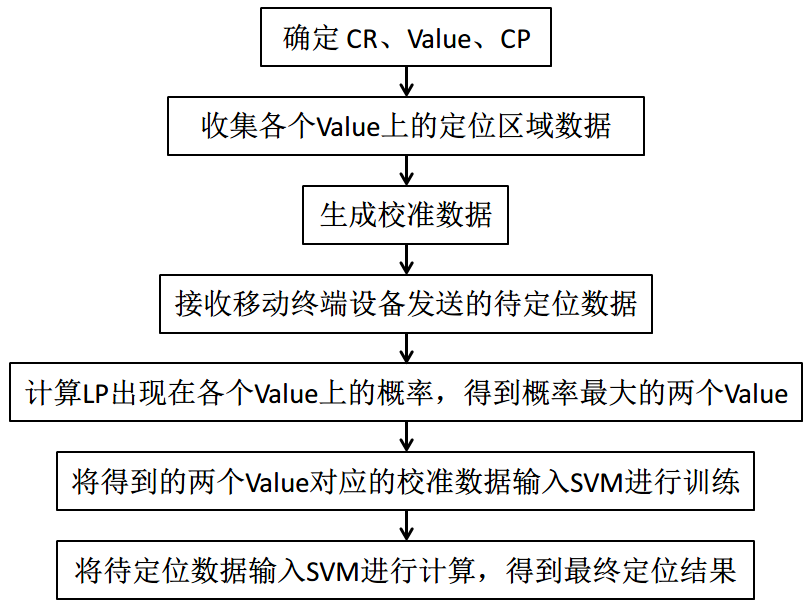
\includegraphics[keepaspectratio, scale=0.3]{no11.png}
  \caption{总体流程示意图\label{fig:no11}} 
\end{figure}
\subsection{确定CR、Value、CP}
\begin{enumerate}
\item 根据实际需求,确定定位空间整体范围。如图\ref{fig:no2}:
  \begin{figure}[!ht]\centering
    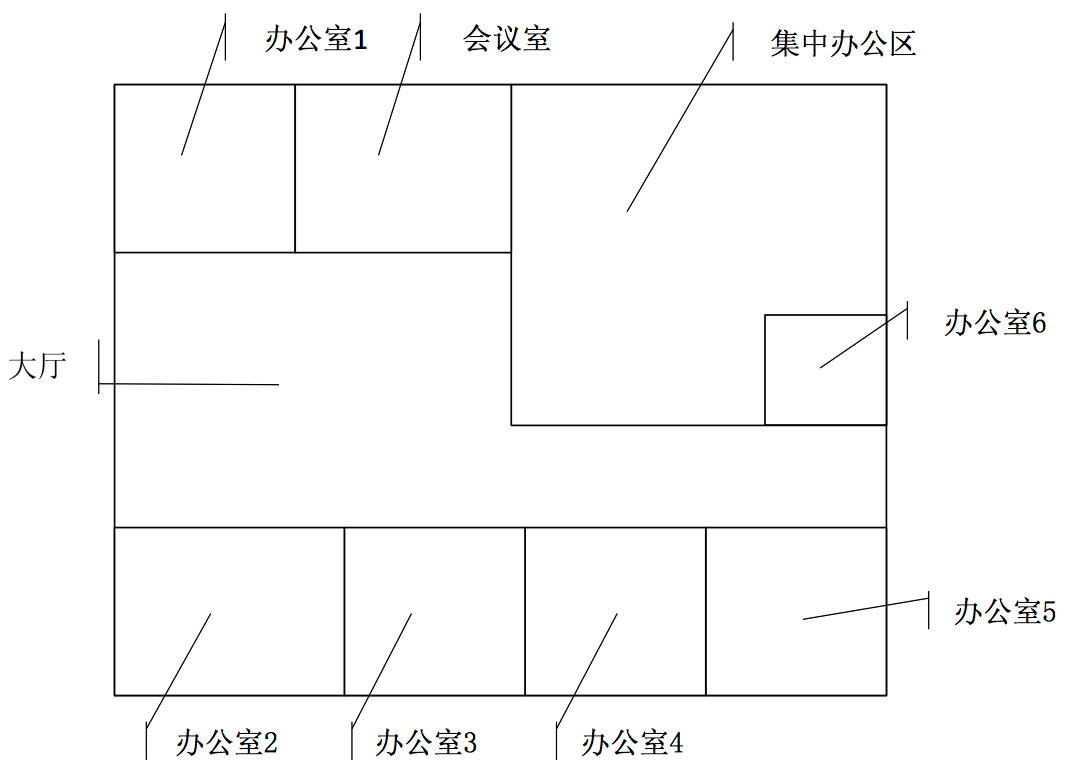
\includegraphics[keepaspectratio, scale=0.2]{no2.png}
    \caption{确定定位空间\label{fig:no2}} 
  \end{figure}
\item 在定位空间内划分出各个定位区域。如图\ref{fig:no3}:
  \begin{figure}[!ht]\centering
    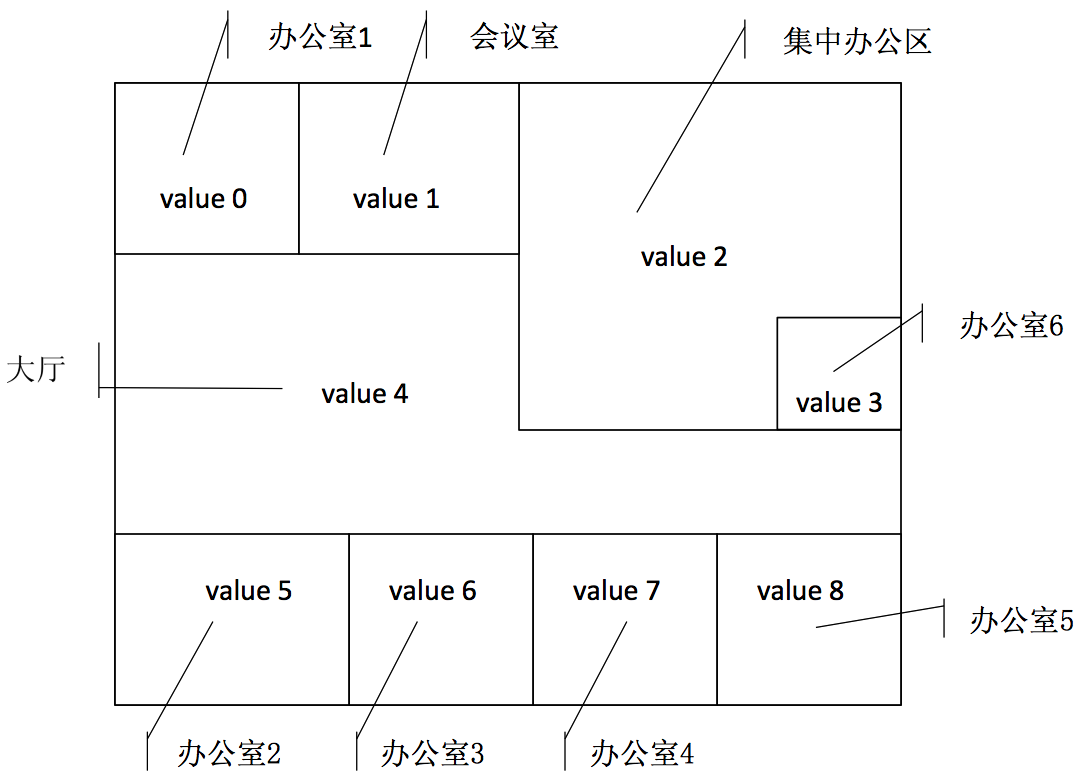
\includegraphics[keepaspectratio, scale=0.2]{no3.png}
    \caption{确定定位区域\label{fig:no3}} 
  \end{figure}
\item 在每个定位区域内确定一个或多个CP。如图\ref{fig:no4}:
  \begin{figure}[!ht]\centering
    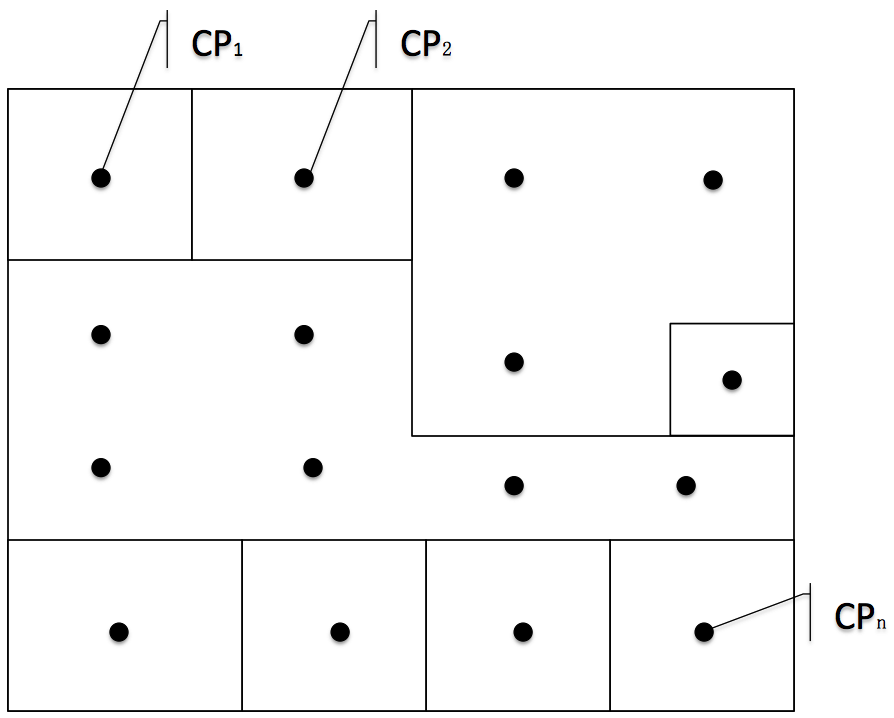
\includegraphics[keepaspectratio, scale=0.2]{no4.png}
    \caption{确定定位校准点\label{fig:no4}} 
  \end{figure}
\end{enumerate}
\subsection{收集各个Value上的定位区域数据}
用移动终端设备,在定位空间内,收集所有定位区域中的多组定位区域数据,将这些数据按定位区域ID,统一保存。
\subsection{生成校准数据}
将收集到的区域定位数据,进行处理,计算出其中每个AP的信号平均值(mRSS)和信号强度值的标准差。按照各AP所对应的区域ID(CP value)组织计算结果,统一保存生成校准数据。如下表所示:
\begin{equation}
  \begin{array}{c|c|c|c}
    Value(n) & AP_{i} & mRSS_{n} & \sigma_{n,i} \\
    \hline
    0 & MAC_{1} & mRSS_{1} & \sigma_{0,1} \\
    0 & MAC_{2} & mRSS_{2} & \sigma_{0,2} \\
    0 & MAC_{3} & mRSS_{3} & \sigma_{0,3} \\
    0 & MAC_{4} & mRSS_{4} & \sigma_{0,4} \\
    0 & MAC_{5} & mRSS_{5} & \sigma_{0,5} \\
    ... & ... & ... & ...\\
    1 & MAC_{1} & mRSS_{1} & \sigma_{1,1} \\
    1 & MAC_{2} & mRSS_{2} & \sigma_{1,2} \\
    1 & MAC_{3} & mRSS_{3} & \sigma_{1,3} \\
    1 & MAC_{4} & mRSS_{4} & \sigma_{1,4} \\
    1 & MAC_{5} & mRSS_{5} & \sigma_{1,5} \\
    ... & ... & ... & ...
  \end{array}
\end{equation}
\subsection{得到移动终端设备的待定位数据}
一个移动终端设备,在定位空间内移动,在不同的位置点上会收集到不同的待定位数据,这些不同的待定位数据都对应不同的待定位点(LP)。将移动终端设备在LP上收集到的带定位数据保存。如下表所示:
\begin{equation}
  \begin{array}{c|c}
    AP_{i} & RSS_{i}\\
    \hline
    MAC_{1} & RSS_{1}\\
    MAC_{2} & RSS_{2}\\
    MAC_{3} & RSS_{3}\\
    MAC_{4} & RSS_{4}\\
    MAC_{5} & RSS_{5}\\
    ... & ...
  \end{array}
\end{equation}
\subsection{计算LP出现在各个Value上的概率,得到概率最大的两个Value}
从校准数据中按照不同Value,依次取出每个Value对应的一组校准数据,将LP的带定位数据与每组校准数据中共有的AP,分别进行正态分布概率计算,计算公式如下:
\begin{equation}
  Pr_{i}=\frac{1}{\sqrt{2\pi}\sigma_{i}}e^{\frac{-(RSS_{i}-mRSS_{i})^{2}}{2\sigma_{i}^{2}}}
\end{equation}
再将计算得到的概率值相加,最终得到了该LP出现在每个Value中的概率。
\par
其中概率值最大的两个Value,就是该LP可能出现的位置范围。

\subsection{将得到的两个Value对应的校准数据输入SVM进行训练}
得到了概率最大的两个Value,说明LP出现在这两个Value中的可能性最大。将LP的待定位数据的AP名和这两个Value对应的校准数据的AP名做交集,得到一组大家都包含的AP。
\par
从LP的待测数据中挑出这个几个共有AP的待定位数据,作为LP的特征数据。
\par
两个Value的校准数据中分别挑出这几个共有的AP校准数据,与该Value的ID一起,作为SVM的特征向量。
\par
将特征向量输入SVM进行训练。 如图\ref{fig:no9}:
\begin{figure}[!ht]\centering
  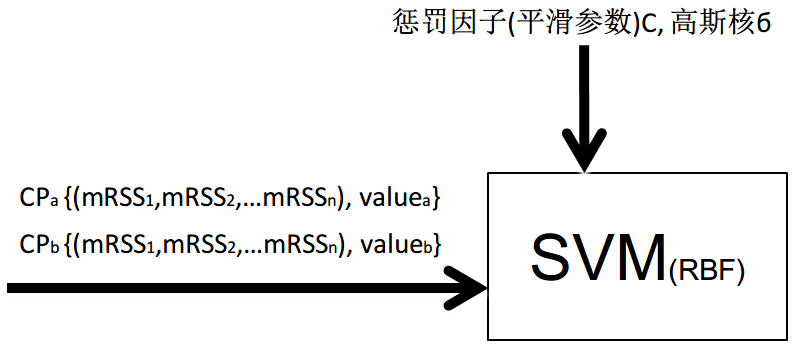
\includegraphics[keepaspectratio, scale=0.3]{no9.png}
  \caption{SVM训练过程\label{fig:no9}} 
\end{figure}

\subsection{将待定位数据输入SVM进行计算,得到最终定位结果}
将LP的特征数据,输入训练完成的SVM,得到一个Value的ID值。该Value所对应的区域就是LP所在的位置。如图\ref{fig:no10}:
\begin{figure}[!ht]\centering
  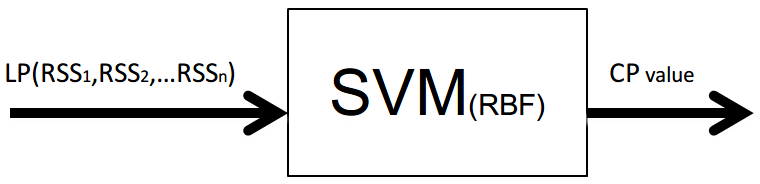
\includegraphics[keepaspectratio, scale=0.3]{no10.png}
  \caption{SVM计算过程\label{fig:no10}} 
\end{figure}
%%%%%%%%%%%%%%%%%%%%%%%%%%%%%%%%%%%%%%%%%%%%%% 

\section{讨论}
在整个WiFi定位过程中,有时会出现无法定位的状况,具体分析有如下两种情况发生:
\begin{enumerate}
\item 待定位数据中的所有AP,不包含在校准数据中。这种情况说民移动终端设备,出现在了定位空间之外的位置,因此无法实现定位。
\item 从待定位数据和校准数据中,无法找出共有的AP,或者共有的AP少于4个。这种情况下无法生成有效的特征向量,因此SVM无法计算。
\item 在某些情行下,待定位数据是SVM不可分类的。这种情况说明移动终端设备出现在两个定位区域的边界上,SVM不能准确计算出移动终端设备的位置。为了比较好的解决这个问题,在使用SVM的过程中可以使用惩罚因子作为计算参数,来提高对不可分类数据的最大识别能力。
\item 对于使用惩罚因子后,依然无法定位的数据,采取失败处理。
\end{enumerate}

%%%%%%%%%%%%%%%%%%%%%%%%%%%%%%%%%%%%%%%%%%%%%% 

\section{技术创新(权利保护)}
\subsection{用边界入口点校准的方法解决WiFi定位功能开关和不同类型设备识别的问题}
本文所阐述的WiFi定位技术,在实际使用的过程中,首先会出现两个必须解决的问题:
\begin{enumerate}
\item 移动终端设备如何判断自身是否进入了一个可定位的空间,并开启定位服务?
\item 移动终端设备如何才能让定位系统知道自身的设备类型?
\end{enumerate}
\par
为了解决以上问题,我们采用边界入口点校准的方法实现。在定位空间的边界上,设置一个或多个入口校准点,所有需要WiFi定位服务的移动终端设备,都必须先到这些入口点进行校准。校准方式有很多种,如手动开启WiFi定位应用,二维码扫描开启WiFi定位应用等。
\par
在开启移动终端设备WiFi定位应用的同时,由于入口校准点是事先约定好的,因此该校准点的定位区域数据也是相对固定的。根据移动终端设备在该点接收到的区域定位数据,就可以判断出这个移动终端设备的WiFi信号识别能力。不同类型的移动终端设备,对于同样的AP,信号强度识别结果是不同的,根据这个特点,便可以基本判断出与这个移动终端设备的最接近的设备类型。

\subsection{用分级校准数据解决不同种类型WiFi设备识别AP信号差异问题}
由于不同类型的移动终端设备,对于同样的AP,信号强度识别结果不同,而一组完整的校准数据是用一台移动终端设备采集的。因此使用一组校准数据,无法实现多种不同类型的移动终端设备,进行准确的WiFi定位。
\par
为了解决这个问题,必须准备多组校准数据,这些数据使用不同类型的移动终端设备进行采集,根据移动终端设备类型分组保存。
\par
当移动终端设备在边界入口点开启WiFi定位应用的同时,根据设备所采集到的入口点的定位区域数据,可以判断出移动终端设备的类型,再根据该移动终端设备类型选择相应的校准数据,最终实现准确的WiFi定位。

\subsection{用共有AP的方法解决SVM训练时AP在识别过程中缺失的问题}
所有移动终端设备,在每次识别AP时都不可能做到绝对准确,因此一台移动终端设备不同时刻识别到的定位区域数据可能会存在不一致的情况。
\par
为了解决以上问题,必须在每次定位时,采用带定位数据与校准数据交集的结果,动态的进行SVM训练,使每次SVM训练用的特征向量中的AP,和LP的特征数据中的AP保证一致。
\par
而每次定位都做SVM训练,计算量非常大,并且已知其中绝大部分计算都是无用的。因此在做SVM计算之前,我们采用概率的方式筛选出LP出现可能最大的两个定位区域。之后之针对这两个定位区域的校准数据做SVM计算,这样大大提高了计算效率,同时保证了定位结果的准确。

%%%%%%%%%%%%%%%%%%%%%%%%%%%%%%%%%%%%%%%%%%%%%% 

\section{应用前景}
WiFi定位技术可以应用在多种领域,主要为行业提供室内定位基础服务。本文阐述的WiFi定位技术,不依赖特定硬件和特殊环境要求,部署应用方便灵活,成本低,可以结合多种具体的业务实现垂直服务。
\subsection{室内定位和导航}
室内定位和导航,是WiFi最主要的应用方式,也是最直接的服务提供模式。
\begin{enumerate}
\item 公共室内空间的位置服务,如商场、超市和大规模的综合购物中心。为了方便顾客找到所需商品位置,或快速找到某个区域(例如卫生间、出口、餐饮区,等等),结合WiFi定位和电子地图技术,实现顾客自身位置确定和导航服务功能。
\item 室内区域流量统计服务,如在商场、超市和大规模的综合购物中心,有时业主需要统计一段时间内,某个区域或所有区域的客流信息,或者某个客流最大的热点区域。结合WiFi定位和电子地图以及大数据技术,可以实现室内区域的流量统计,顾客使用移动设备上的WiFi定位客户端软件,经过的路径会推送至服务器,服务器端根据统计整理,最后分析出某个或所有区域的客流数据。
\end{enumerate}
\subsection{地理围栏}
地理围栏是一个新兴的移动互联网服务概念,其主要目的是实现互联网应用和移动设备位置信息的结合。
\begin{enumerate}
\item 设备位置开启移动应用。当移动设备进入某个特定区域后,便自动开启一些应用软件。这种服务适合应用在商场导购,医院就医指导,机场火车站等公共服务场所。
\item 特定移动应用的使用范围。移动设备上的某些软件,只能在某些特定的环境中才可以使用。这种服务适合公司企业,用来实现现代移动化的企业管理和自动化办公。当员工进入企业办公区域后,相关工作的信息服务和业务软件才可以工作,保证了企业数据的安全,也将企业管理简单有效的实现。
\end{enumerate}
\subsubsection{移动设备防盗}
某些非个人使用的移动设备,如餐厅的点餐设备,高级场馆的自助服务设备,都是为了本地服务存在的。为了防止个别人将其私自带出,又要实现该设备的自由使用,就必须采用一种防盗的技术做应用保证。本文阐述的WiFi定位技术,可以划出移动设备的安全范围,当设备离开这个安全区域后,便可以通过报警、监控和追踪等方式及时发现并处理。
\subsubsection{区域信息安全}
信息隔离,是信息安全中的一项重要内容,指信息内容与信息的有效区域之间的对应关系。采用本文阐述的WiFi定位技术,可以通过软件安全策略,规定信息的安全范围,当移动设备需要读取某些带有安全级别的数据时,会根据移动设备所处的位置进行操作合法性判断,当发现移动设备所处的位置不合法时,便会组织数据的读取。对于已经读取到的数据,当设备离开该数据的安全区域后,通过软件安全策略谁自动删除该数据,保证数据存在的有效范围与数据的安全范围一致。
\subsubsection{地理信息隔离}
移动设备的最大特点是可以随身携带,可以随时随地的产生数据,如照相、笔记、下载或应用软件生成数据。利用本文所阐述的WiFi定位技术,可以在产生数据的同时,将数据与其产生时的位置做关联。无论在以后的搜索查找,或是统计,位置信息会提供跟多的有效途径,版主使用者对数据的管理。也可以将数据的存储或显示方式,与位置信息关联,是某些数据只在特定位置区域是才可以被操作。
\subsection{游戏}
电子游戏的场景通常是虚拟的空间,但是随着技术的发展,电子游戏的实现也可以利用现实空间。本文阐述的WiFi定位技术,可以实现真实空间在设备上的体现,电子游戏的方式也就从单一的虚拟空间扩展到了真实空间,游戏玩家除了操作设备,还需要亲身行动来完成游戏。这样的组合不仅扩展了电子游戏的功能,甚至可以改变电子游戏的传统运行模式。
%%%%%%%%%%%%%%%%%%%%%%%%%%%%%%%%%%%%%%%%%%%%%% 

\end{document}
